% !Mode:: "TeX:UTF-8:Main"
% gif command (hope it still works ...)
% magick -density 160 -delay 35 -loop 0 XXXX.pdf XXXX.gif
% this here slower, around 105!
% magick -density 160 -delay 100 -loop 0 XXXX.pdf XXXX.gif

% delay 105 => 100/105 FPS
% Needed: 25 FPS
% => increase number of pages by 25/(100/105) = 26.25
% => show each page 26 times

\PassOptionsToPackage{svgnames,x11names}{xcolor}
\documentclass{beamer}
\usepackage[T1]{fontenc} % or fontspec if lualatex is wanted ...
\setbeamertemplate{navigation symbols}{}
\usepackage{tikz}
\setbeamertemplate{background}{}
\setbeamertemplate{background canvas}{}
\ExplSyntaxOn
\cs_set_eq:NN\intmod\int_mod:nn
\ExplSyntaxOff
\newcommand\tipperaryduck{
\includegraphics[scale=0.6,page=\inteval{\intmod{\x}{19}+1}]{irishflag}~}

\begin{document}
\foreach\x in {1,2,...,200}{%
\begin{frame}
\begin{tikzpicture}[remember picture,overlay]
% Background image
\node[at=(current page.center)]{%
	%\includegraphics[height=\paperheight]{thames1}
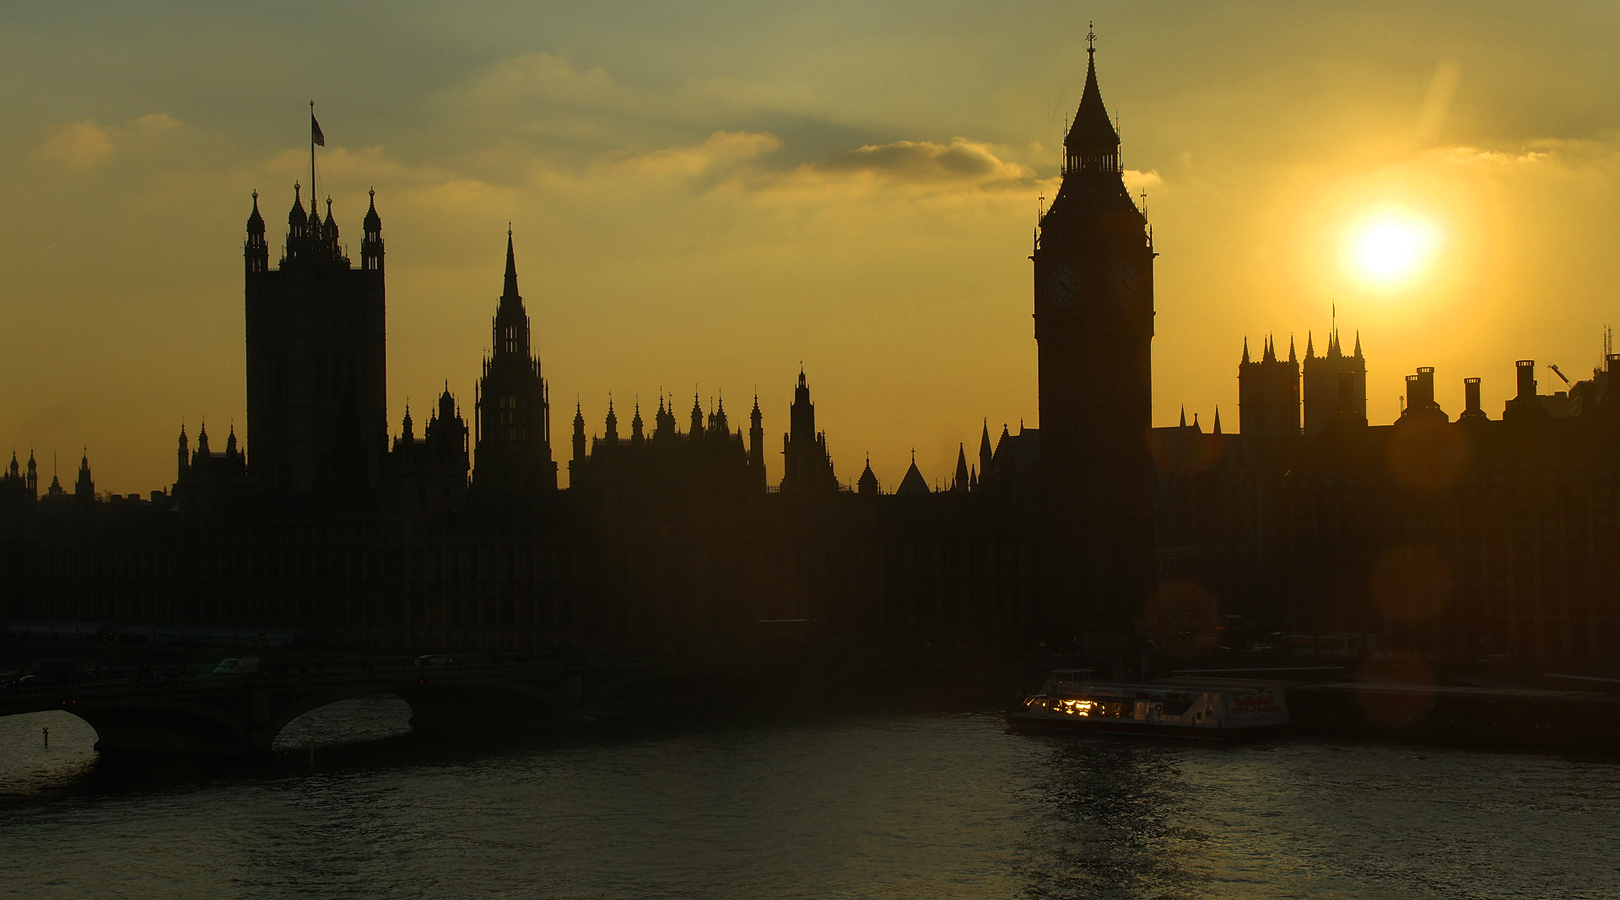
\includegraphics[height=\paperheight]{thames2}
};	
% Image credit of background
\node[at=(current page.south),yshift=0.25cm,text width=\paperwidth,font=\tiny,align=center,white]{%
    \url{https://commons.wikimedia.org/wiki/File:London_Parliament_on_the_River_Thames_(6812540384).jpg}
};
\end{tikzpicture}

\vspace*{5cm}
\hspace*{\dimexpr\linewidth-\fpeval{\x*0.006}\linewidth}%
\makebox[0pt][l]{%
\tipperaryduck\tipperaryduck\tipperaryduck\tipperaryduck\tipperaryduck\tipperaryduck\tipperaryduck\tipperaryduck\tipperaryduck\tipperaryduck\tipperaryduck
}
\end{frame}
}
\end{document}
